\section{流动反应器中流体的混合}


\begin{frame}
    \frametitle{流动反应器中流体的混合}

    离析流模型，其基本假定是流体粒子从进入反应器起到离开反应器止，粒子之间不发生任何物质交换，或者说粒子之间不产生混合，这种状态称为完全离析，即各个粒子都是孤立的，各不相干的。如果粒子之间发生混合又是分子尺度的，则这种混合称为微观混合。当反应器不存在离析的流体粒子时，微观混合达到最大，这种混合状态称为完全微观混合或最大微观混合。介乎两者之间则称为部分离析或部分微观混合，即两者并存。
    \begin{itemize}
        \item 完全离析(宏观流体)    
        \item 完全微观混合(微观流体)
        \item 部分微观混合
    \end{itemize}

\end{frame}


\begin{frame}
    \frametitle{流动反应器中流体的混合}

    混合状态的不同，将对化学反应产生不同的影响。设浓度分别为$c_\mathrm{A1}$和$c_\mathrm{A2}$而体积相等的两个流体粒
子，在其中进行$\alpha$级不可逆反应。
    \begin{itemize}
        \item 完全离析
        
        \[
            \langle r_\mathrm{A}\rangle  = \frac{1}{2}(r_\mathrm{A1} + r_\mathrm{A2}) = \frac{k}{2}(c_\mathrm{A1}^{\alpha} + c_\mathrm{A2}^{\alpha})
        \]
        \item 完全微观混合
        
        \[
            \langle r_\mathrm{A}' \rangle  = k[(c_\mathrm{A1} + c_\mathrm{A2})/2]^{\alpha}
        \]
    \end{itemize}
    这就说明了微观混合程度不同将会对化学反应的速率发生影响。
    
    $\langle r_\mathrm{A}\rangle$与$\langle r_\mathrm{A}' \rangle$的大小与$\alpha$值有关。

\end{frame}


\begin{frame}
    \frametitle{流动反应器中流体的混合}

    \begin{minipage}{0.48\linewidth}
        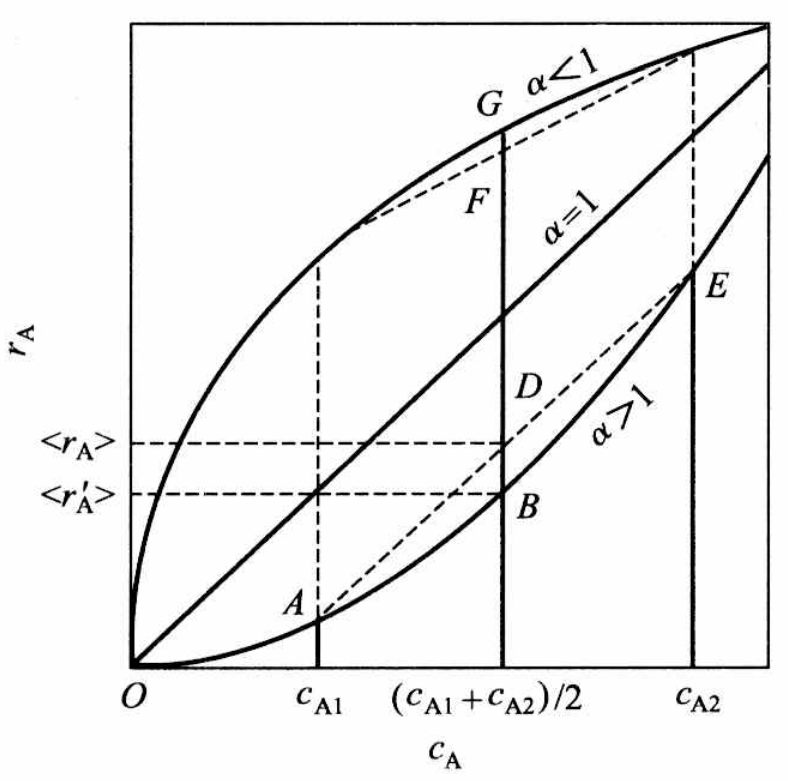
\includegraphics[width=\linewidth]{figures/fig5.25.png}
    \end{minipage}\hfill
    \begin{minipage}{0.48\linewidth}
        \begin{itemize}
            \item $\alpha=1$时，$\langle r_\mathrm{A}\rangle = \langle r_\mathrm{A}' \rangle$
            \item $\alpha>1$时，$\langle r_\mathrm{A}\rangle > \langle r_\mathrm{A}' \rangle$
            
            微观混合使平均反应速率下降。
            \item $\alpha<1$时，$\langle r_\mathrm{A}\rangle < \langle r_\mathrm{A}' \rangle$
            
            微观混合使平均反应速率加快。
        \end{itemize}
    \end{minipage}
    
\end{frame}


\begin{frame}
    \frametitle{微观混合对反应器工况的影响}

    \begin{itemize}
        \item 间歇反应器
        
        任何时刻下，间歇反应器中所有流体粒子均具有相同的停留时间，因而其组成亦应相同。所以微观混合的程度不影响反应器的工况。
        \item 活塞流反应器
        
        同一横截面上所有流体粒子停留时间相同，组成自然也相同，所以，微观混合的程度对活塞流反应器的工况不产生影响。
        \item 全混流反应器
        
        由于同一横截面上流体粒子的停留时间不同，其组成也就不同，于是，除一级反应外，微观混合的程度将影响反应器的工况。这种影响随着停留时间分布的不同而不同，返混程度越严重，微观混合程度的影响越大。
    \end{itemize}

\end{frame}


\begin{frame}
    \frametitle{微观混合对反应器工况的影响}

    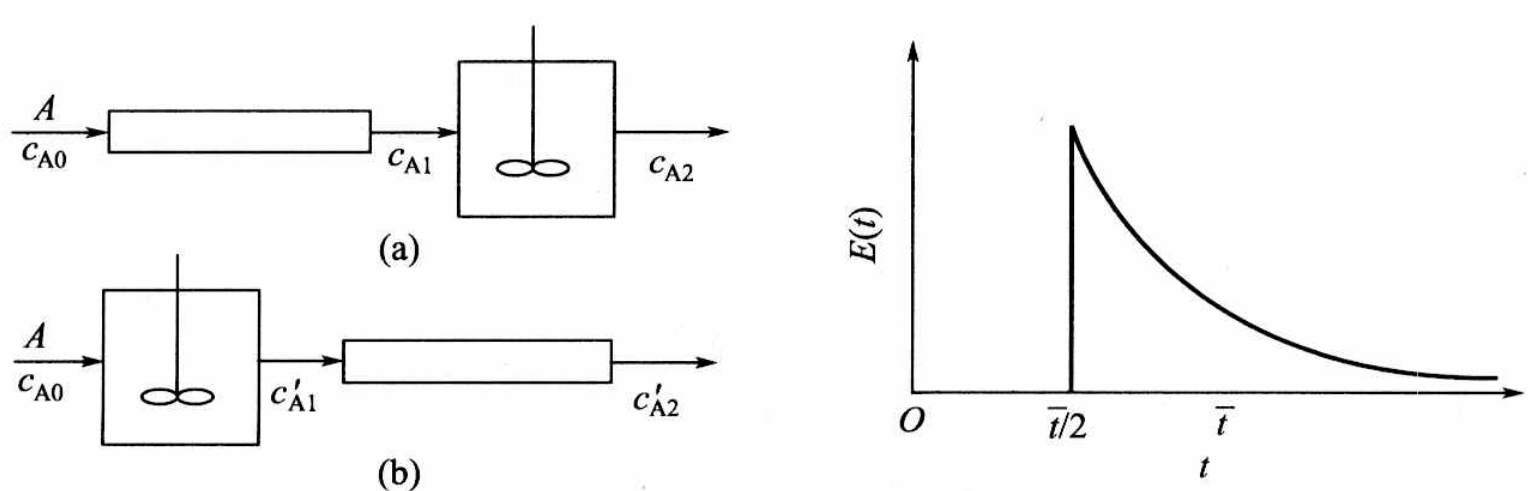
\includegraphics[width=\linewidth]{figures/fig5.26.png}

    (a) (b) 两种连接方式，停留时间分布相同，如果微观混合的程度也相同，是否两者的工况也相同呢？

\end{frame}


\begin{frame}[t]
    \frametitle{}

    \begin{example}
        如图所示两个串联反应器系统，在相同的温度及空时下进行同样的反应。若相串联的全混流反应器和活塞流反应器的空时均等于1 min，进口流体中$c_\mathrm{A0} = \SI{1}{kmol/m^3}$，试分别计算这两种串联情况所达到的转化率。假设所进行的反应为（1）一级反应；（2）二级反应，反应温度下两者的反应速率常数分别为\SI{1}{(min^{-1})}及\SI{1e-3}{m^3/(mol.min)}。        
    \end{example}
    \begin{figure}
        \centering
        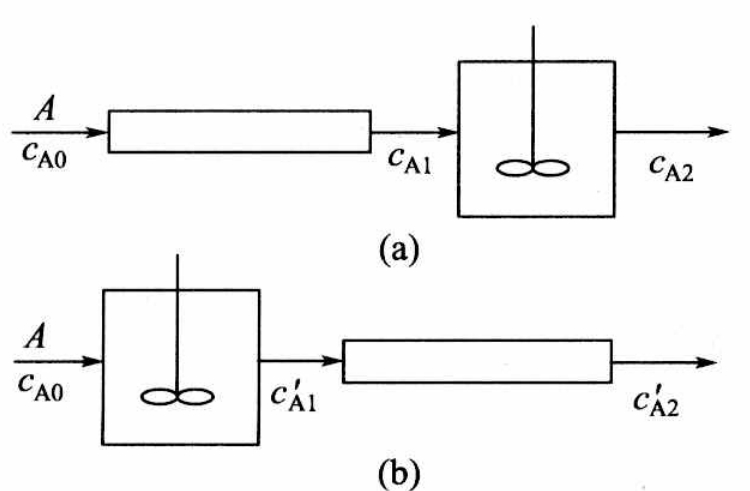
\includegraphics[width=.4\linewidth]{figures/fig5.26a.png}
    \end{figure}

\end{frame}